\subsection{Network Representation Learning}
\label{subsec:nrl}

Representation learning methods have the goal of generating low-dimensional, continuous vector representations for entities in high-dimensional, heterogeneous data sets (e.g., images, text sequences, etc.).
More specifically, network representation learning, also known as \ac{KGE}, learns representations of nodes and edges from \ac{KG}s in continuous vector spaces that can be used in downstream machine learning tasks such as edge prediction, entity clustering, and entity disambiguation~\cite{Wang2017}.
Several methods inspired by linear algebra, deep learning, and natural language processing have arisen in previous years as shown in Table~\ref{tab:kgem_examples}.

\begin{table}
    \centering
    \caption{Examples of three types of \ac{KGEM}s}\label{tab:kgem_examples}
    \begin{tabular}{ l l l }
        \hline
        Type & Model & Reference \\
        \hline
        \multirow{6}{*}{Translational Distance Models}
        & Structured Embedding & ~\cite{Bordes2011}  \\
        & TransE & ~\cite{Bordes2013} \\
        & Unstructured Model & ~\cite{Bordes2014} \\
        & TransH & ~\cite{Wang2014} \\
        & TransR & ~\cite{Lin2015} \\
        & TransD & ~\cite{Ji2015} \\
        \hline
        \multirow{4}{*}{Semantic Matching Models}
        & RESCAL & ~\cite{Nickel2011} \\
        & ERMLP & ~\cite{Dong2014} \\
        & DistMult & ~\cite{Yang2014}  \\
        & ConvE & ~\cite{Dettmers2017} \\
        \hline
        \multirow{4}{*}{Random-Walk Models}
        & DeepWalk & ~\cite{Perozzi2014} \\
        & Gat2Vec & ~\cite{Sheikh2018} \\
        & node2vec & ~\cite{Grover2016} \\
        & edge2vec & ~\cite{Gao2018} \\
        & LINE & ~\cite{Tang2015} \\
        \hline
    \end{tabular}
\end{table}

\subsubsection{Translational Distance Models}

Each translational distance model learns entity and relation embeddings in euclidean space by defining two things: 1) an equation relating the corresponding embeddings with the models' hyperparameters and 2) a distance-based measure of the plausibility of a given triple $f_r$~\cite{Wang2017}.

An example of an established translational distance model is TransE~\cite{Bordes2013}.
It models a class of relation \textit{r} as the translation from a head entity $h$ (i.e., the subject of a triple) to a tail entity $t$ (i.e., the object of a triple) in a representative euclidean space as $h + r \approx t$.
It measures the plausibility of a given the following scoring function:

\begin{equation}\label{eq:trans_e_scoring_function}
    f_r(h,t) = - \|h + r - t\|
\end{equation}

The closer the embedding of the tail is to the sum of the head and relation embeddings, the higher is the probability that the triple is correct.
However, because TransE is limited in modeling $1-N$, $N-1$, and to $N-M$ relations, several extensions have been proposed (e.g., TransH, TransR, and TransD).

\subsubsection{Semantic Matching Models}

Unlike translational distance models, semantic matching models use similarity-based scoring functions that measure the plausibility of a given triple based on the "latent semantics" of the entities and relations~\cite{Wang2017}.
An example of an established semantic matching model is RESCAL~\cite{Nickel2011}.
It represents each entity as a vector and each relation as a matrix, $M_r$, that encodes pairwise interactions between the head and tail entities of a triple, using the following scoring function:

\begin{equation}\label{eq:rescal_scoring_function}
    f_r(h,t) = h^{T} M_{r} t
\end{equation}

Both translational distance models and semantic matching models can be trained using the margin ranked loss in order to maximize the difference between true (i.e., positive) and false (i.e., negative) triples.

\begin{equation}\label{eq:margin_ranked_loss}
    L = \sum_{}^{}(f_r(h^{'},t^{'}) - f_r(h,t) + \lambda )_+,
\end{equation}

\subsubsection{Random Walk Models}

Random walk models generate embeddings for nodes in knowledge graphs by applying the concepts from natural language models (e.g., SkipGram, Word2Vec, and GloVE) to random walks.
The first, \textit{DeepWalk}~\cite{Perozzi2014}, used random walks to train a SkipGram~\cite{Mikolov2013} model in which the random walks were considered as sentences and nodes were considered as words.
Because SkipGram is a language model that maximizes the co-occurrence probability of words in the same window, the resulting node vectors reflect the local structure of the input \ac{KG} (Figure~\ref{fig:deepwalk_embedding}).
It is further rationalized by the observation that the distribution of nodes' appearances in random walks mirrors that of words in free text~\cite{Perozzi2014}.

\begin{figure}
    \captionsetup{format=plain}
    \makebox[\textwidth]{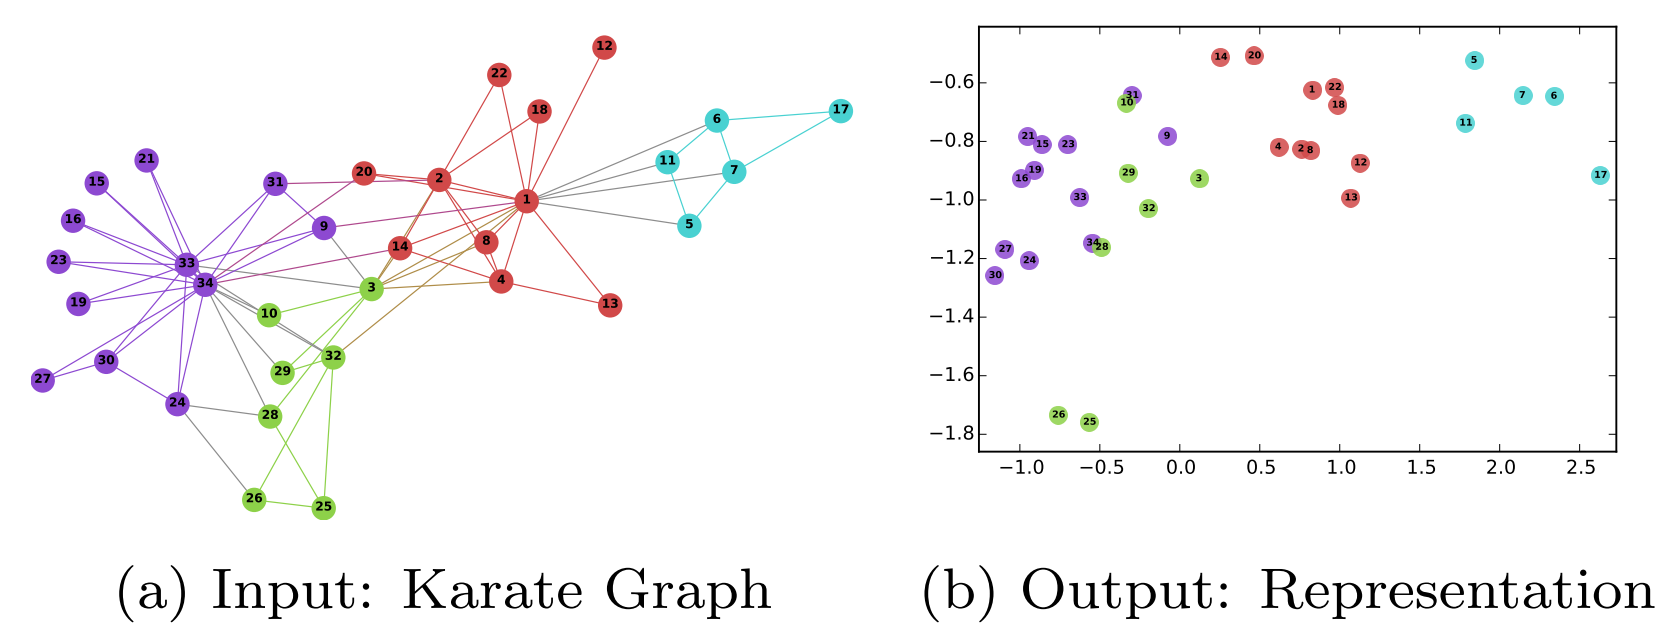
\includegraphics[width=120mm]{figures/deepwalk_embedding.png}}
    \caption{\textit{DeepWalk} produces embeddings that reflect the community structure of the underlying \ac{KG}. Figure adapted from ~\cite{Perozzi2014}}
    \label{fig:deepwalk_embedding}
\end{figure}

Biological knowledge encoded in many of the previously mentioned formats (e.g., \ac{BioPAX}, \ac{SBML}) can be directly translated into \ac{KG}s to which network representation learning can be applied.
The following subsection describes two of such applications in drug discovery.
